\documentclass[12pt]{article}

\usepackage{amssymb,amsmath,amsfonts,eurosym,geometry,ulem,graphicx,caption,color,setspace,sectsty,comment,footmisc,caption,natbib,pdflscape,subfigure,array,hyperref,natbib}

\normalem
\usepackage [english]{babel}
\usepackage [autostyle, english = american]{csquotes}
\usepackage{float}
\usepackage{indentfirst}
\usepackage{etoolbox}

\usepackage{lscape}
\usepackage{setspace}
\usepackage{stackrel}
\newtheorem{theorem}{Theorem}
\newtheorem{corollary}[theorem]{Corollary}
\newtheorem{proposition}{Proposition}
\newtheorem{lemma}{Lemma}
\newtheorem{assumption}{Assumption}
\newenvironment{proof}[1][Proof]{\noindent\textbf{#1.} }{\ \rule{0.5em}{0.5em}}

\newtheorem{hyp}{Hypothesis}
\newtheorem{subhyp}{Hypothesis}[hyp]
\renewcommand{\thesubhyp}{\thehyp\alph{subhyp}}

\newcommand{\red}[1]{{\color{red} #1}}
\newcommand{\blue}[1]{{\color{blue} #1}}

\newcolumntype{L}[1]{>{\raggedright\let\newline\\arraybackslash\hspace{0pt}}m{#1}}
\newcolumntype{C}[1]{>{\centering\let\newline\\arraybackslash\hspace{0pt}}m{#1}}
\newcolumntype{R}[1]{>{\raggedleft\let\newline\\arraybackslash\hspace{0pt}}m{#1}}

\newcommand\blfootnote[1]{%
  \begingroup
  \renewcommand\thefootnote{}\footnote{#1}%
  \addtocounter{footnote}{-1}%
  \endgroup
}
\allowdisplaybreaks
\geometry{left=1.0in,right=1.0in,top=1.0in,bottom=1.0in}
\linespread{1.25}

\usepackage{pgf}
\usepackage{tikz}
\usetikzlibrary{arrows,automata}

\begin{document}

\title{Interactive Projection Tool for COVID-19 Interventions \\ \emph{Technical Documentation}}
\author{COVID-19 Statistics, Policy modeling and Epidemiology Collective (C-SPEC)}
\date{}
\maketitle

\section{Model}

\subsection{Model Structure}

The model uses the following structure, with susceptible individuals (\(S\)) progressing to an exposed state (\(E\)), and then moving to either an undetected symptomatic infected state (\(UI\)) or an undetected asymptomatic state (\(UA\)). From there, symptomatic infected individuals can either die or recover, or move to a detected symptomatic state (\(DI\), and asymptomatic individuals can only recover or move to a detected asymptomatic state (\(DA\)). Detected individuals can then recover or die (if they are symptomatic). (Note that \(\lambda=\beta S I/N\), discussed below.)

\begin{figure}[H]
\centering
\scalebox{1.1}{
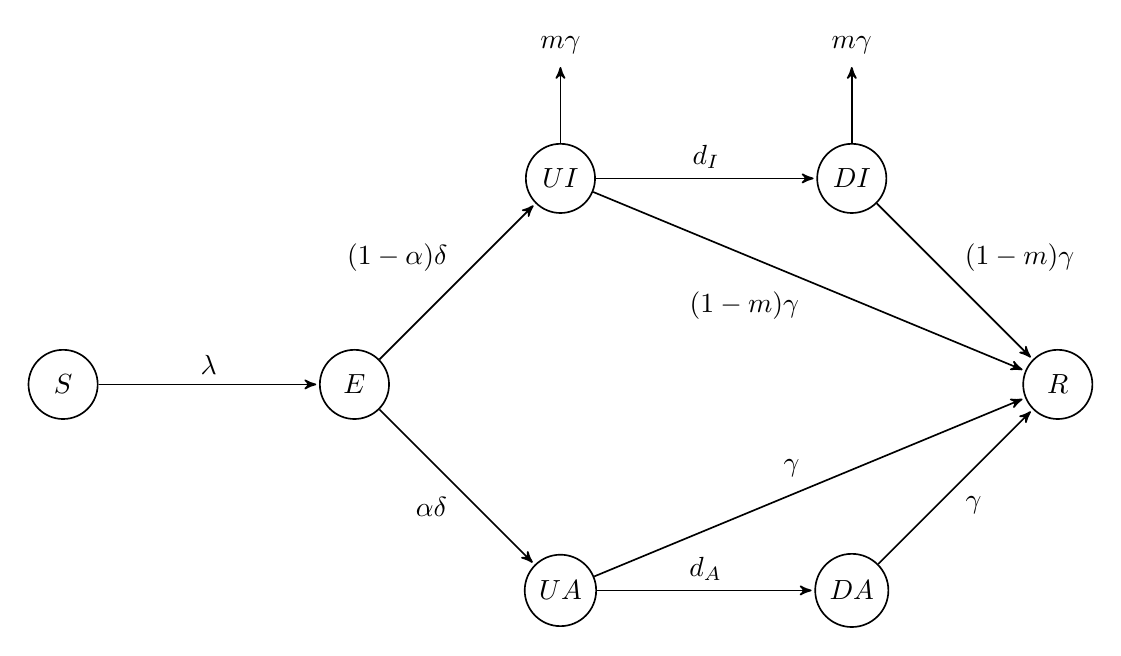
\begin{tikzpicture}[->,>=stealth',shorten >=1pt,auto,node distance=3.7cm,
                    semithick]
  \tikzstyle{every state}=[fill=white,draw=black,text=black]

  \node[state]         (S)                    {$S$};
  \node[state]         (E) [right of=S] {$E$};
  \node[state]         (J) [above right of=E] {$UI$};
  \node[state]         (B) [below right of=E] {$UA$};
  \node[state]         (I) [right of=J] {$DI$};
  \node[state]         (A) [right of=B] {$DA$};
	\node[state]         (R) [above right of=A] {$R$};

  \path (S)  edge  node {\(\lambda\)} (E)
        (E)  edge  node {\((1-\alpha)\delta\)} (J)
             edge  [below left] node {\(\alpha\delta\)} (B)
        (J) edge  node {\(d_I\)} (I)
             edge [below left] node {\((1-m)\gamma\)} (R)
        (B) edge  node {\(d_A\)} (A)
             edge  node {\(\gamma\)} (R)
        (I) edge  node {\((1-m)\gamma\)} (R)
        (A) edge [below right] node {\(\gamma\)} (R);
  \path [draw, ->] (I.north) -- ++(0,1cm) node[above] {\(m\gamma\)};
  \path [draw, ->] (J.north) -- ++(0,1cm) node[above] {\(m\gamma\)};
\end{tikzpicture}}
    \caption{Model Structure}
    \label{fig:model}
\end{figure}

\subsection{Baseline Specification}

The population is stratified by age into three groups: $i = \{< 20, 20-64, 65+\}$. Then, let \(\beta_{ij}=v_{ij} p k_{Si}k_{Ij}\) be the effective contact rate between susceptible and symptomatic individuals, and let \(\beta_{ij_A}=v_{ij}p\kappa k_{Si}k_{Ij}\) be the effective contact rate between susceptible and asymptomatic individuals. Here, \(v_{ij}\) is the number of daily contacts with individuals in group \(j\) per person in group \(i\), \(p\) is the probability of infection per contact between a susceptible and infected individual, \(\kappa\) is the relative reduction in the effective contact rate when the contact is with an asymptomatic individual, compared to a symptomatic individual, \(k_{Si}\) is the relative susceptibility of individuals in age group \(i\), and \(k_{Ij}\) is the relative infectiousness of individuals in age group \(j\). Then, the model is defined by the following system of differential equations (where \(N_i = S_i + E_i + UA_i + DA_i + UI_i + DI_i + R_i\)):
\begin{align*}
\frac{\partial S_i}{\partial t} &= -\sum_{j=1}^3 \beta_{ij} S_i \frac{UI_j+k_{Det}DI_j}{N_j} - \sum_{j=1}^3 \beta_{ij_A} S_i \frac{UA_j+k_{Det}DA_j}{N_j} \\
\frac{\partial E_i}{\partial t} &= \sum_{j=1}^3 \beta_{ij} S_i \frac{UI_j+k_{Det}DI_j}{N_j} + \sum_{j=1}^3 \beta_{ij_A} S_i \frac{UA_j+k_{Det}DA_j}{N_j}- \delta E_i \\
\frac{\partial UA_i}{\partial t} &= \alpha_i\delta E_i  - (k_{Rep,i}r_A+\gamma) UA_i \\
\frac{\partial DA_i}{\partial t} &= k_{Rep,i}r_A UA_i - \gamma DA_i \\
\frac{\partial UI_i}{\partial t} &= (1-\alpha_i)\delta E_i - (k_{Rep,i}r_I + \gamma)  UI_i\\
\frac{\partial DI_i}{\partial t} &= k_{Rep,i}r_A UI_i - \gamma DA_i\\
\frac{\partial R_i}{\partial t} &= (1-m_i)\gamma (UI_i + DI_i) + \gamma (UA_i + DA_i)
\end{align*}

In addition to \(\beta_{ij}\) defined above, \(k_{Det}\) is the relative reduction in social contacts for individuals with a detected infection, \(\delta\) is the rate of progression out of the exposed state, \(\alpha_i\) is the proportion of infections that are asymptomatic for age group \(i\), \(k_{Rep,i}\) is the relative detection (i.e., ``reporting'') rate for individuals in age group \(i\), \(r_A\) is the detection rate for asymptomatic infections, \(r_I\) is the detection rate for symptomatic infections, \(\gamma\) is the rate of progression from infected to recovered or death, and \(m_i\) is the proportion of individuals in age group \(i\) who die once they exit the infected state.

\subsection{Social Distancing Intervention}

In order to model a social distancing intervention, an additional set of ``social distancing'' compartments are added to the model -- a constant fraction \(s\) of each age stratum are split between the social distancing and baseline contact compartments. The effective contact rates between individuals in the social distancing compartments, and between individuals in the baseline contact and social distancing compartments, are reduced by a constant fraction -- the effective contact rates for these interactions become \(\beta_{ij}^{SD}=e v_{ij} p k_{Si}k_{Ij}\) and \(\beta_{ij_A}^{SD}=e v_{ij}p\kappa k_{Si}k_{Ij}\), where \(e\in[0,1]\). Then, the model is defined by the following system of differential equations, where the social distancing compartments are notated with the \(SD\) superscript:
\begin{align*}
		\frac{\partial S_i}{\partial t} &= -\sum_{j=1}^3 \beta_{ij} S_i \frac{UI_j+k_{Det}DI_j}{N_j} - \sum_{j=1}^3 \beta_{ij_A} S_i \frac{UA_j+k_{Det}DA_j}{N_j} \\
		&-\sum_{j=1}^3 \beta_{ij}^{SD} S_{i} \frac{UI_{j}^{SD}+k_{Det}DI_{j}^{SD}}{N_{j}^{SD}} - \sum_{j=1}^3 \beta_{ij_A}^{SD} S_i \frac{UA_{j}^{SD}+k_{Det}DA_{j}^{SD}}{N_{j}^{SD}} \\
		\frac{\partial E_i}{\partial t} &= \sum_{j=1}^3 \beta_{ij} S_i \frac{UI_j+k_{Det}DI_j}{N_j} + \sum_{j=1}^3 \beta_{ij_A} S_i \frac{UA_j+k_{Det}DA_j}{N_j} \\
		&+\sum_{j=1}^3 \beta_{ij}^{SD} S_{i} \frac{UI_{j}^{SD}+k_{Det}DI_{j}^{SD}}{N_{j}^{SD}} + \sum_{j=1}^3 \beta_{ij_A}^{SD} S_i \frac{UA_{j}^{SD}+k_{Det}DA_{j}^{SD}}{N_{j}^{SD}}- \delta E_i \\
		\frac{\partial UA_i}{\partial t} &= \alpha_i\delta E_i  - (k_{Rep,i}r_A+\gamma) UA_i \\
		\frac{\partial DA_i}{\partial t} &= k_{Rep,i}r_A UA_i - \gamma DA_i \\
		\frac{\partial UI_i}{\partial t} &= (1-\alpha_i)\delta E_i - (k_{Rep,i}r_I + \gamma)  UI_i\\
		\frac{\partial DI_i}{\partial t} &= k_{Rep,i}r_A UI_i - \gamma DA_i\\
		\frac{\partial R_{i}}{\partial t} &= (1-m_i)\gamma (UI_i + DI_i) + \gamma (UA_i + DA_i)\\
		\frac{\partial S_i^{SD}}{\partial t} &= -\sum_{j=1}^3 \beta_{ij}^{SD} S_{i}^{SD} \frac{UI_j+k_{Det}DI_j}{N_j} - \sum_{j=1}^3 \beta_{ij_A}^{SD} S_{i}^{SD} \frac{UA_j+k_{Det}DA_j}{N_j} \\
		&-\sum_{j=1}^3 \beta_{ij}^{SD} S_{i}^{SD} \frac{UI_{j}^{SD}+k_{Det}DI_{j}^{SD}}{N_{j}^{SD}} - \sum_{j=1}^3 \beta_{ij_A}^{SD} S_{i}^{SD} \frac{UA_{j}^{SD}+k_{Det}DA_{j}^{SD}}{N_{j}^{SD}}\\
		\frac{\partial E_{i}^{SD}}{\partial t} &= \sum_{j=1}^3 \beta_{ij}^{SD} S_{i}^{SD} \frac{UI_j+k_{Det}DI_j}{N_j} + \sum_{j=1}^3 \beta_{ij_A}^{SD} S_{i}^{SD} \frac{UA_j+k_{Det}DA_j}{N_j} \\
		&+\sum_{j=1}^3 \beta_{ij}^{SD} S_{i}^{SD} \frac{UI_{j}^{SD}+k_{Det}DI_{j}^{SD}}{N_{j}^{SD}} + \sum_{j=1}^3 \beta_{ij_A}^{SD} S_{i}^{SD} \frac{UA_{j}^{SD}+k_{Det}DA_{j}^{SD}}{N_{j}^{SD}} - \delta E_{i}^{SD} \\
		\frac{\partial UA_{i}^{SD}}{\partial t} &= \alpha_i\delta E_{i}^{SD}  - (k_{Rep,i}r_A+\gamma) UA_{i}^{SD} \\
		\frac{\partial DA_{i}^{SD}}{\partial t} &= k_{Rep,i}r_A UA_{i}^{SD} - \gamma DA_{i}^{SD} \\
		\frac{\partial UI_{i}^{SD}}{\partial t} &= (1-\alpha_i)\delta E_{i}{SD} - (k_{Rep,i}r_I + \gamma)  UI_{i}^{SD}\\
		\frac{\partial DI_{i}^{SD}}{\partial t} &= k_{Rep,i}r_A UI_{i}^{SD} - \gamma DA_{i}^{SD}\\
		\frac{\partial R_{i}^{SD}}{\partial t} &= (1-m_i)\gamma (UI_{i}^{SD} + DI_{i}^{SD}) + \gamma (UA_{i}^{SD} + DA_{i}^{SD})
\end{align*}

\section{Baseline Parameter Values}

The interactive projection tool uses the baseline parameter values in the table below as the default settings. Some of these values were set based on available data or similar models -- these sources are also described below.

\begin{table}[H]
\begin{tabular}{p{0.15\textwidth}  p{0.65\textwidth} p{0.2\textwidth}}
\textbf{Parameter}             & \textbf{Description} & \textbf{Value}  \\\hline
\(n_i(0)+n_{i}^{SD}\) & Age Distribution at \(t=0\) & \((0.25, 0.59, 0.16)\)\\
\(v_{ij}\) & Average number of contacts with individuals in group \(j\) per person in group \(i\) &  (See Below)\\
\(p\) & Probability of transmission given contact with an infectious person & 0.05 \\
\(\kappa\)& Relative infectiousness of asymptomatic individuals & 0.375 \\
\(k_{Si}\) & Relative susceptibility of individuals in age group \(i\) & \(1,1,1\) \\
\(k_{Ii}\) & Relative infectiousness of individuals in age group \(i\) & \(1,1,1\) \\
\(k_{Det}\) & Relative contact reduction for infected individuals & 0.5 \\
\(\frac{1}{\delta}\) & Average length of the incubation period    & 5 days \\
\(\alpha_i\) & Proportion of cases in age group \(i\) that do not go on to experience symptoms & \((0.75, 0.3, 0.3)\) \\
\(k_{Rep,i}\) & Relative detection rate for individuals in age group \(i\) & \((1,1,1)\)\\
\(r_A\) & Detection rate for asymptomatic infections & 0.01 detections per day\\
\(r_I\) & Detection rate for symptomatic infections & 0.1 detections per day\\
\(\frac{1}{\gamma}\) & Average duration of infection to recovery or death &  5 days\\
\(m_i\) & Mortality risk for group \(i\) & \((0, 0.01, 0.1)\) \\
\(s\) & Fraction of population in social distancing compartments & 0.01 \\
\(e\) & Relative reduction in contact rates for individuals in socially distancing compartments & 0 \\\hline
\end{tabular}
\caption{Baseline Parameters Values}
\end{table}

\subsection{Age distribution}

We assume an age distribution representative of the United States with 25\% of the population under 20, 59\% between 20 and 64, and 16\% at least 65 \citep{censusbureau}.  While individual municipalities may not reflect these averages, we find that these values are similar across major metropolitan areas (Figure \ref{fig:age.dist}), and we do not formally model uncertainty around these parameters.

\begin{figure}[H]
    \centering
    \includegraphics{dem.pdf}
    \caption{Age distribution by location.  Due to rounding errors, total may not sum to 100\%.  (Source: American Community Survey 2018 via \citet{noauthor_population_2019} and \citet{noauthor_census_2020}).}
    \label{fig:age.dist}
\end{figure}

\subsection{Contact rates between strata}

Very limited primary data exists on age-stratified contacts in the US. Therefore, we rely on methods that project contact rates derived from surveys in other contexts and US demographics. We use the age-structured contact matrix for the US estimated by \cite{prem2017projecting}, which was derived by projecting the POLYMOD \cite{mossong2008social,mossong2017polymod} survey data to US demographics \cite{prem2017projecting}. Since we are interested in 3 broad age-classes, we bin the projected contacts according to US Census Bureau age-distribution estimates for 2018 (\cite{censusbureau}). This provided the following baseline contact matrix, where \(v_{ij}\) is the average number of daily contacts with individuals in group \(j\) per person in group \(i\) (i.e., \(v_{12}\) represents the number of daily contacts where an infectious individual in group 2 could infect a susceptible individual in group 1):

\begin{equation*}
    \begin{bmatrix}
9.7619 & 2.2706 & 0.2923\\
6.6876 & 10.3334 & 0.8853\\
0.9157 & 1.0141 & 1.2495
\end{bmatrix}
\end{equation*}

\subsection{Probability of Transmission}
The probability of transmission is determined by calibrating the model to an empirical estimate of the basic reproduction number \(R_0\). Both \citet{li_early_2020} and \citet{Riou_R0} estimate \(R_0\) at 2.2; following \citet{peak_modeling_2020} we assume a 95\% confidence interval of (1.46, 3.31) and calibrate the transmission probability to the \(R_0\) estimate of 2.2. The calibrated value for the transmission probability per contact is 0.05.

Additionally, we assume that the rate of transmission from asymptomatic individuals is systematically lower than the transmission probability from symptomatic individuals. There is no empirical estimate for this reduction in transmission, however, so we assume that the transmissibility of asymptomatic infection is 37.5\% the rate of symptomatic infection. This assumption reflects a middle ground between the 50\% value used by \citet{Zhao2020} (which is similar to the estimate for influenza) and the 25\% value used by \citet{Prem2020} (which they derived from \citet{Liu2020}).

\subsection{Age-specific mortality rates}

We assume that the mortality risks among symptomatic individuals are 0\%, 1\%, and 10\% for the 0-19, 20-64, and 65+ age groups, respectively. These assumptions are consistent with estimates from \citet{riou_adjusted_2020}, which adjusts crude fatality rates from Hubei province, China to account for delayed mortality and unidentified cases. They estimate that the case fatality risk is less than 0.05\% among individuals 19 years of age and younger, between 0.19\% and 2.7\% for individuals between 20-59 years old, and is at least 9.5\% for individuals older than 60. (For comparison, the \citet{ChinaEpiWG} reports the crude case fatality risk from all reported Chinese cases through February 11, 2020, as 0.10\% for individuals aged 0-19 (1 deaths out of 965 cases), 0.98\% for ages 20-59 (193 deaths out of 19,790 cases), and 5.96\% for ages 60 and older (829 deaths out of 13,909) -- the high proportion of unreported mild cases leads to a lower adjusted CFR for the younger age groups, and the delayed mortality leads to a higher adjusted CFR for the older age group.)

\subsection{Proportion of asymptomatic infections}

We assume that, for individuals 20 years and older, 30\% of infections are asymptomatic. This assumption is supported by findings from \citet{nishiura2020}, which found that 30.8\% (95\% CI: 7.7, 53.8) of infected individuals among Japanese citizens evacuated from Wuhan, China were asymptomatic. Similarly, \citet{mizumoto_estimating_2020} estimate that, among individuals on the Diamond Princess Cruise ship, 17.9\% (95\% CI: 15.5, 20.2) were asymptomatic.

There is less available data on the proportion of asymptomatic infections among individuals younger than 20 years, but we assume that 75\% of such infections are asymptomatic. This assumption is also supported by the data from the Diamond Princess Cruise ship -- among the 6 cases detected in individuals under 20 years old as of Februrary 20, 2020, 4 of the cases were asymptomatic \citep{Russell2020}.

\subsection{Incubation and Latent period}

We assume an incubation period of 5 days, consistent with the existing literature. \citet{li_early_2020} reported a mean incubation period of 5.2 days in the first 425 confirmed patients from Wuhan, China; \citet{linton_2020} estimate a mean period of 5.6 days for patients in China (both inside and outside Wuhan); \citet{lauer_2020} estimates the median incubation period at 5.1 days for patients outside Hubei province, China; while \citet{xu_2020} reports a slightly lower median period of 4 days for patients in Zhejiang province, China, and \citet{backer_incubation_2020} reports a slightly higher mean period of 6.4 days for travelers from Wuhan, China.

Additionally, we assume that the incubation and latent periods coincide and that there is no pre-symptomatic infectious period. This is likely not an accurate assumption, given reports of pre-symptomatic transmission, but unfortunately no data is available on the length of the latent period itself. This assumption will be revisited and updated in the model as more data becomes available.

\subsection{Duration of Infectious Period}

There is limited evidence available on the duration of the infectious period. We assume the duration of the infectious period is 5 days, and that it coincides with the entire duration of disease. This assumption aligns with \citet{Prem2020}, which modeled a length of both 3 and  7 days.


\section{Modeling Interventions}

The interactive projection tool allows users to model different types of interventions by changing the baseline parameters listed above, and evaluate the impact on different outcome measures. For example, in order to model social distancing interventions, the fraction of the population in the social distancing compartments (\(s\)) can be increased and the relative reduction in contacts by individuals in those compartments (\(e\)) can be decreased. Similarly, in order to model treatments that reduce the mortality risk, the values for \(m_i\) can be changed across the population.

\setlength\bibsep{0pt}
\bibliographystyle{aer}
\bibliography{lib}

\end{document}
